\section{Results}
\label{sec:results}

\todo{Add more results (matter of running more experiments, mostly)}

\subsection{Multi-model Translations}
Figure~\ref{fig:accuracy_multi_model_wikis} shows the accuracy of the multi-model translations, both for models trained on 100 and 400 dimensions. We used the same training set of translations to train the matrix on, and both language models are trained on respectively the Dutch and English Wikipedia.

An interesting observation is that the accuracy at all levels (top 1, top 5 and top 10) starts off lower for models trained at 400 dimensions. However, at the biggest training set, each level is better than the corresponding level at 100 dimensions. This suggests a form of overfitting; the translation matrix might be overfitted on the translation samples.

\todo{There's also a dip towards the end. Check if that's still there if we run it with differently split test/training data sets.}

\begin{figure}[ht!]
  \centering 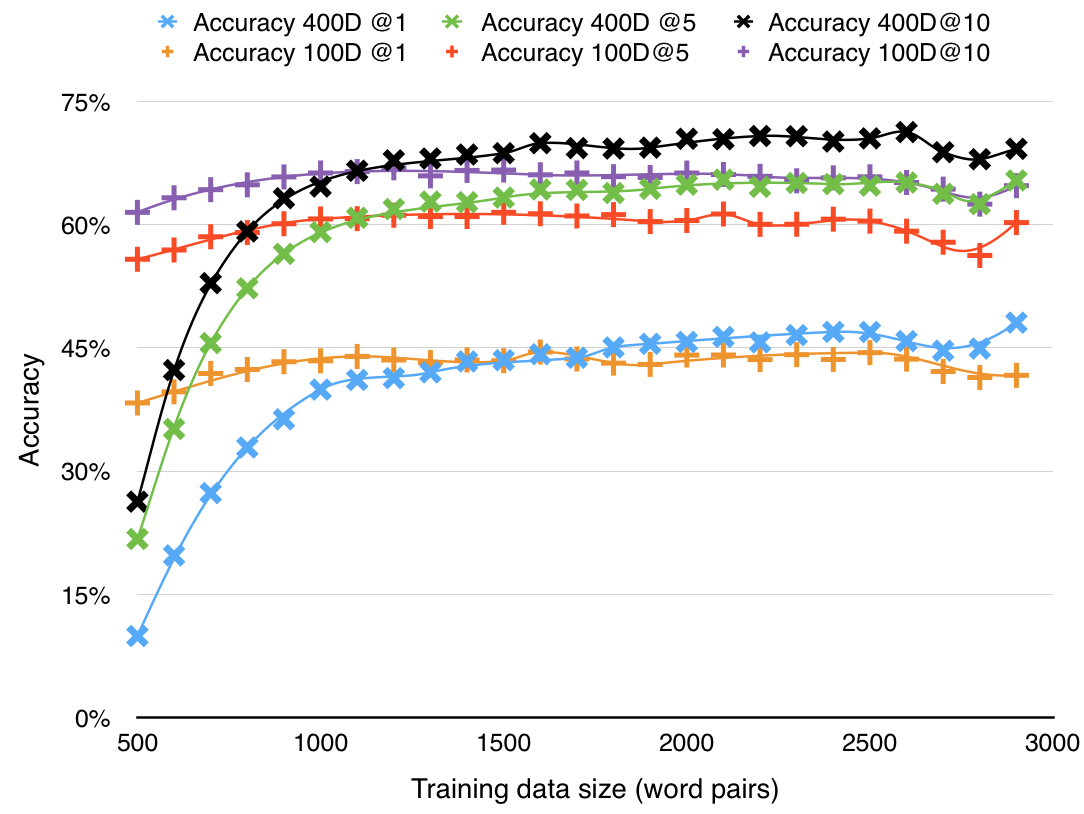
\includegraphics[width=\linewidth]{images/accuracy_multi_model_wikis}
  \caption{Accuracy for multi-model translations, trained on Dutch and English wiki. 'x' marks denote dimensionality 400, '+' marks dimensionalty 100.}
  \label{fig:accuracy_multi_model_wikis}
\end{figure}

\subsection{Single-model Translations}
\subsubsection{Using Relations}

\subsubsection{Using Translation Matrix}
\todo{repeat experiment from multi model section, but use bothwiki 100 and bothwiki 400 as language models}
